\documentclass[12pt]{article}

\usepackage[margin=1in]{geometry}
\usepackage[T1]{fontenc}
\usepackage[utf8]{inputenc}
\usepackage{lmodern}
\usepackage{microtype}
\usepackage{setspace}
\usepackage{amsmath,amssymb,amsthm,mathtools}
\usepackage{array}
\usepackage{booktabs}
\usepackage{graphicx}
\usepackage{subcaption}
\usepackage{hyperref}
\usepackage{natbib}
\usepackage{enumitem}
\usepackage{float}

\hypersetup{
  colorlinks=true,
  linkcolor=blue,
  urlcolor=blue,
  citecolor=blue
}

\onehalfspacing
\setlength{\parindent}{0pt}
\setlength{\parskip}{0.7em}

\newtheorem{proposition}{Proposition}
\newcolumntype{L}[1]{>{\raggedright\arraybackslash}p{#1}}

\title{\textbf{Repeated Wet Years, Flood Exposure, and Local Economic Adjustment: Evidence from Minnesota Counties}}
\author{Brendyn Beasley}
\date{April 2026}

\begin{document}

\maketitle

\begin{abstract}
This paper uses annual county-level weather variation to study how local economies adjust to repeated wet years under existing flood exposure in Minnesota. I assemble a county-year panel for all 87 Minnesota counties over 2011--2023 by harmonizing NOAA weather records, FEMA flood-risk measures, Census and IRS demographic data, BLS and QCEW labor-market outcomes, QWI labor-flow data, BEA personal income and county GDP, Census building permits, County Business Patterns, and USDA NASS crop outcomes. The empirical design uses county and year fixed effects and extends the baseline with distributed lags, three-year moving averages, and precipitation-by-flood-risk interactions. Because the panel is short, the estimates are best interpreted as evidence on repeated wet years and local exposure, not as a direct estimate of long-run climate-trend effects.

The strongest evidence is concentrated in three margins: permitting, construction-sector output, and agricultural productivity. Wetter county-years are associated with fewer permit units, lower construction GDP, and significantly lower corn and soybean yields. At the sample interquartile range of annual precipitation, the baseline estimates imply roughly 20 percent fewer permit units, 6.7 percent lower construction GDP, and 6 to 7 percent lower corn and soybean yields. QWI labor-flow estimates provide supporting evidence of local disruption through lower total-private hiring and higher construction separation rates, while total county GDP is comparatively muted. Employment is negative in the baseline models but weakens once county-specific trends are added, and demographic outcomes are more specification-sensitive throughout. Overall, the paper is best read as evidence that repeated wet years in a flood-exposed inland state are most clearly associated with weaker construction activity, lower construction-sector output, and lower crop productivity.
\end{abstract}

\textbf{Keywords:} weather variation; flood exposure; local adjustment; housing supply; agriculture; Minnesota

\textbf{JEL Codes:} Q54; R11; R23; J61

\section{Introduction}

Understanding how annual weather variation shapes local adjustment under existing flood exposure is a central question in regional and applied economics. Much of the policy conversation emphasizes coastal flooding, sea-level rise, wildfire, or extreme heat in large metropolitan areas. Yet economically meaningful local stress can also emerge in inland states when repeated wet years interact with flood exposure, infrastructure strain, agricultural disruption, and housing-market frictions. This paper studies whether those forms of weather-related pressure are visible in annual local adjustment across Minnesota counties, with particular attention to construction activity and agricultural productivity.

Minnesota is an informative setting for this question for three reasons. First, its counties vary meaningfully in precipitation, temperature, inland flood risk, and economic structure. Second, the state is large enough to exhibit substantial regional heterogeneity but compact enough to support a complete, harmonized county-year panel. Third, Minnesota is an inland Upper Midwest state rather than a canonical coastal climate case. If weather-related local stress is economically visible here under existing flood exposure, then the scope of regional adjustment is likely broader than the most familiar coastal or Sun Belt narratives imply.

This paper sits at the intersection of several literatures. In climate economics, a large body of work uses weather variation to study how climate conditions affect output, productivity, and local welfare \citep{dell2014,hsiang2016,hsiang2017}. In agriculture, the evidence points to large productivity consequences from adverse weather and only partial adaptation in U.S. farming \citep{schlenker2009,burke2016}. In regional and urban economics, local adjustment is often understood through migration, labor-market reallocation, and housing supply \citep{blanchard1992,cattaneo2016,glaeser2005,saiz2010}. The distinctive contribution here is to connect those margins within one county-year panel for an inland state where precipitation and flood exposure, rather than coastal hazards, appear to be the dominant weather-related stresses.

The paper is therefore best understood as a study of annual weather realizations interacting with fixed local exposure rather than as a direct estimate of secular climate change over multi-decade horizons. The identifying variation comes from within-county year-to-year fluctuations in precipitation and temperature, evaluated against persistent differences in flood exposure. That design is informative about how repeated wet years line up with local adjustment margins under existing flood risk, but it should not be read as an estimate of thirty-year climate normals or long-run global damage functions.

The paper asks three connected questions. First, do wetter county-years reduce local construction activity and construction-sector output? Second, do the same conditions lower agricultural productivity in a state where crop exposure remains economically important? Third, do labor-market and demographic outcomes move in the same direction as supporting evidence of broader local adjustment? These questions are motivated by a simple idea: adverse weather does not need to produce a dramatic collapse in every market to matter economically. It can instead show up most clearly in sectors that are especially exposed to wet conditions and only more weakly in downstream labor and demographic outcomes.

The paper makes three contributions. First, it assembles a broad Minnesota county-year panel that links annual weather variation and flood exposure to construction, sectoral output, agriculture, labor markets, and migration within a common empirical frame. Second, it evaluates those outcome families using a layered econometric design that moves from baseline county fixed effects to lagged, persistent, and heterogeneity specifications. Third, it uses that common framework to distinguish between the paper's strongest outcome blocks, especially construction and agriculture, and weaker but still informative supporting margins in labor and demographics. The result is a paper that is formal enough to generate theory-linked predictions and disciplined interpretation while remaining credible for the available county-year data.

The paper also speaks to adjacent literatures on local adaptation, regional adjustment, and housing supply. Its distinctive feature is not a single outcome or a single dataset, but the ability to trace weather-related stress across construction activity, sectoral output, agricultural productivity, and selected labor and demographic outcomes within one consistently constructed county panel.

The main empirical result is that precipitation is the dominant adverse weather margin in the Minnesota data. The clearest headline results are fewer building permits, lower construction GDP, and lower corn and soybean yields in wetter county-years. In magnitude terms, moving from the 25th to the 75th percentile of annual precipitation in the sample is associated with about 19.9 percent fewer permit units, 6.7 percent lower construction GDP, and 6 to 7 percent lower corn and soybean yields in the baseline fixed-effects estimates. QWI labor-flow estimates add further supporting evidence: wetter years are associated with lower total-private hiring and higher construction separation rates. Employment is also lower in the baseline fixed-effects models, but that result weakens once county-specific trends are added; the demographic estimates are supportive but more sensitive to alternative specifications throughout. Temperature is not irrelevant, but it is less central for the main real-activity outcomes and appears more strongly in BEA income measures, especially per capita income. The clearest heterogeneity result is that precipitation is more harmful for employment in counties with higher inland flood risk. Taken together, these patterns suggest that repeated wet conditions are most clearly associated with weaker building activity, lower construction-sector output, and lower crop productivity, with labor and demographic margins moving in the same direction less consistently.

The remainder of the paper proceeds as follows. Section 2 develops a local adjustment framework that motivates the empirical design. Section 3 presents the layered econometric system. Section 4 describes the data and descriptive patterns. Section 5 reports the main findings, beginning with construction and sectoral productivity and then turning to labor and demographic outcomes as supporting evidence. Sections 6 through 8 discuss interpretation, implications, and conclusion.

\section{A Local Adjustment Framework}

This paper does not attempt to estimate a full general equilibrium model of the Minnesota economy or to recover deep structural parameters such as substitution elasticities or policy-invariant migration preferences. The county panel is better suited to a disciplined reduced-form framework with an explicit economic mapping from annual weather conditions to observable local outcomes. In that sense, the paper follows the broader principle that modeling, identification, and empirical interpretation should remain internally consistent even when the design is not fully structural. The goal of this section is to formalize that mapping and show how the empirical specifications follow from it.

Let county-level weather stress in county $c$ and year $t$ be summarized by
\begin{equation}
A_{ct} = \psi_T T_{ct} + \psi_P P_{ct} + \psi_{PR}\left(P_{ct}\times R_c\right).
\end{equation}
Here, $T_{ct}$ is annual average temperature, $P_{ct}$ is annual precipitation, and $R_c$ is baseline flood risk. The object $A_{ct}$ is not directly observed; it is a latent index of local weather-related pressure that combines production-side disruption and amenity-side deterioration. Higher precipitation can raise disruption costs through flood exposure, infrastructure strain, and construction delays. Higher temperature can reduce local productivity or residential desirability, even if its effects are weaker or more outcome-specific.

The key conceptual step is that county outcomes adjust through distinct margins. Household sorting is one margin, construction is another, and labor demand is a third. Let inward migration, building activity, and economic activity respond to weather stress as follows:
\begin{equation}
\text{InMig}_{ct} = f_H(A_{ct}), \qquad \text{Build}_{ct} = f_B(A_{ct}), \qquad Y_{ct} = f_Y\!\left(A_{ct}, \text{InMig}_{ct}, \text{Build}_{ct}\right).
\end{equation}

These mappings say that annual weather conditions can directly affect local outcomes, but they can also affect them indirectly by changing who moves in and how much new construction occurs. A hotter or wetter year can make a county less attractive at the same time that it makes building activity more difficult or more costly. Lower inflows and weaker construction then feed into broader employment and income outcomes.

For empirical work, I use a linearized version of this system:
\begin{align}
\text{InMig}_{ct} &= \alpha_0 + \alpha_1 A_{ct} + \mu_c + \tau_t + \varepsilon_{ct}, \\
\text{Build}_{ct} &= \delta_0 + \delta_1 A_{ct} + \mu_c + \tau_t + \nu_{ct}, \\
\text{Emp}_{ct} &= \gamma_0 + \gamma_1 A_{ct} + \gamma_2 \text{InMig}_{ct} + \gamma_3 \text{Build}_{ct} + \mu_c + \tau_t + \omega_{ct}.
\end{align}

Equations (3) through (5) should not be read as a fully identified simultaneous system. Rather, they provide an organizing structure for the paper's evidence. The empirical analysis first estimates the reduced-form effect of weather variation on migration, construction, employment, and related outcomes. It then asks whether the pattern of results across those outcome families is consistent with the adjustment logic in equations (3) through (5).

\begin{proposition}
If precipitation lowers county attractiveness for households and raises disruption costs for local construction and labor demand, then in a county fixed-effects framework the reduced-form effect of precipitation on population growth, net in-migration, building permits, and employment should be negative on average. Moreover, if flood exposure amplifies the disruptive effect of precipitation, then the absolute value of the precipitation effect should be larger in counties with higher baseline flood risk.
\end{proposition}

The proposition is intentionally modest. It does not claim that each outcome must respond equally strongly or in the same year. Instead, it provides a sign prediction for the central outcomes and a heterogeneity prediction for flood-prone counties. The empirical sections of the paper test those predictions directly.

\section{Econometric Framework}

\subsection{Baseline County Fixed-Effects Model}

The baseline empirical model is
\begin{equation}
Y_{ct} = \beta_T T_{ct} + \beta_P P_{ct} + \alpha_c + \gamma_t + X_{ct}'\delta + \varepsilon_{ct}.
\end{equation}

The dependent variable $Y_{ct}$ varies across outcome families: population growth, IRS net migration, unemployment, log employment, log income, log permit units, log construction establishments, and related measures. County fixed effects $\alpha_c$ absorb all time-invariant county characteristics, including geography, baseline industrial composition, and persistent institutional differences. Year fixed effects $\gamma_t$ absorb shocks common to all counties in a given year, including statewide macroeconomic conditions. Standard errors are clustered at the county level to allow for arbitrary serial correlation within counties over time.

The vector $X_{ct}$ is deliberately parsimonious. In some specifications it is omitted entirely, so that identification comes from within-county changes in annual weather conditions net of county and year effects. This choice reflects the logic of the project: the goal is not to maximize the number of controls, but to isolate how deviations in annual weather conditions within a county are associated with deviations in county outcomes.

\subsection{Outcome-Specific Mapping}

The general fixed-effects equation can be specialized to the paper's main outcome families:
\begin{align}
\text{PopGrowth}_{ct} &= \beta_T^P T_{ct} + \beta_P^P P_{ct} + \alpha_c + \gamma_t + \varepsilon_{ct}^P, \\
\text{NetMig}_{ct} &= \beta_T^M T_{ct} + \beta_P^M P_{ct} + \alpha_c + \gamma_t + \varepsilon_{ct}^M, \\
\text{Employment}_{ct} &= \beta_T^E T_{ct} + \beta_P^E P_{ct} + \alpha_c + \gamma_t + \varepsilon_{ct}^E, \\
\text{Permits}_{ct} &= \beta_T^B T_{ct} + \beta_P^B P_{ct} + \alpha_c + \gamma_t + \varepsilon_{ct}^B.
\end{align}

These equations formalize the empirical spirit of the paper: compare counties to themselves over time and ask whether hotter or wetter years are associated with weaker demographic and economic outcomes.

\subsection{Persistence and Distributed Lags}

The empirical results suggest that the most important weather relationships are not always purely contemporaneous. Employment, in particular, appears more sensitive to lagged and accumulated precipitation than to same-year precipitation alone. To capture that persistence, I estimate distributed-lag models of the form
\begin{equation}
Y_{ct} = \sum_{k=0}^{K}\beta_k P_{c,t-k} + \sum_{k=0}^{K}\theta_k T_{c,t-k} + \alpha_c + \gamma_t + \varepsilon_{ct},
\end{equation}
with special attention to $K=2$. In practice, the paper presents contemporaneous, one-year lag, and three-year average specifications. This design allows weather stress to persist rather than requiring the entire effect to occur in the same calendar year.

\subsection{Multi-Year Weather Exposure}

To capture accumulated exposure more directly, I also estimate moving-average specifications:
\begin{equation}
Y_{ct} = \theta_T \text{TempMA}_{ct}^{(3)} + \theta_P \text{PrecMA}_{ct}^{(3)} + \alpha_c + \gamma_t + \varepsilon_{ct},
\end{equation}
where
\begin{align}
\text{TempMA}_{ct}^{(3)} &= \frac{1}{3}\left(T_{ct}+T_{c,t-1}+T_{c,t-2}\right), \\
\text{PrecMA}_{ct}^{(3)} &= \frac{1}{3}\left(P_{ct}+P_{c,t-1}+P_{c,t-2}\right).
\end{align}

These moving-average measures are useful when local adjustment is gradual. If wetter conditions erode economic momentum through delayed construction, household sorting, or business responses, then multi-year exposure may be more informative than a same-year weather shock alone.

\subsection{Flood-Risk Heterogeneity}

The paper's most substantive interaction question is whether precipitation is more harmful in counties with higher baseline flood risk. Let $R_c$ denote a standardized FEMA overall risk score or inland flood risk score. The heterogeneity equation is
\begin{equation}
Y_{ct} = \beta_T T_{ct} + \beta_P P_{ct} + \beta_{TR}\left(T_{ct}\times R_c\right) + \beta_{PR}\left(P_{ct}\times R_c\right) + \alpha_c + \gamma_t + \varepsilon_{ct}.
\end{equation}

Because $R_c$ is time-invariant over the sample, its main effect is absorbed by county fixed effects and is not separately identified. The interaction term $\beta_{PR}$ is therefore the key object of interest. A negative estimate of $\beta_{PR}$ implies that wetter years are associated with larger adverse outcome shifts in counties with higher baseline flood exposure.

\subsection{A Dynamic Law of Motion for Local Momentum}

To give the paper a forward-looking interpretation without pretending to estimate a full dynamic equilibrium, I also interpret the reduced-form estimates through a simple law of motion for local economic momentum:
\begin{equation}
g_{c,t+1} = \rho g_{ct} + \phi_T T_{ct} + \phi_P P_{ct} + \phi_{PR}\left(P_{ct}\times R_c\right) + \eta_{c,t+1}.
\end{equation}
Here, $g_{ct}$ can represent employment growth, income growth, or construction growth. Equation (13) formalizes the idea that county outcomes are persistent and that annual weather conditions can shift the path of local momentum.

Under this interpretation, expected future activity satisfies
\begin{equation}
E_t\!\left[g_{c,t+\tau}\right]
= \rho^\tau g_{ct}
 + \sum_{s=0}^{\tau-1}\rho^s\left[\phi_T T_{c,t+\tau-1-s} + \phi_P P_{c,t+\tau-1-s} + \phi_{PR} P_{c,t+\tau-1-s}R_c\right].
\end{equation}

This is not a structural forecasting equation used for estimation in the paper. Instead, it provides an interpretation of why lagged and moving-average weather measures are economically meaningful: if weather shocks affect county momentum and that momentum is persistent, then the consequences of wet years should unfold over more than one period.

\subsection{What This Paper Does Not Claim}

The framework above is formal, but it is intentionally not a full general equilibrium model. The paper does not impose a CES production function, solve a Bellman equation for forward-looking migration or investment choice, or calibrate a statewide equilibrium with market clearing across sectors. Those would be interesting extensions, but they would require richer identifying assumptions and data than are currently available. The contribution here is instead a serious reduced-form county-economy framework: clearly stated equations, theoretically motivated persistence and heterogeneity, and a mechanism-oriented map linking annual weather conditions to migration, construction, employment, and income outcomes.

\section{Data and Measurement}

The analysis combines multiple sources into a harmonized Minnesota county-year panel. NOAA Climate at a Glance provides the core weather variables: annual average temperature and annual precipitation. FEMA's National Risk Index provides baseline hazard measures, especially the overall county risk score and the inland flood risk score. Census county population estimates provide annual population totals and population growth rates. IRS county migration files provide inflow, outflow, and net migration measures.

The labor and income extensions add BLS local area unemployment rates, QCEW employment and wage measures, QWI annual labor-flow outcomes, and both BEA CAINC1 personal income data and BEA county GDP data. Housing and construction outcomes come from the Census Building Permits Survey and County Business Patterns, while FHFA county house-price indices are available as a supplementary housing-price series. Agriculture outcomes come from USDA NASS county-year data on corn, soybean, and spring wheat acreage and yields.

All sources are harmonized using five-digit county FIPS codes. This design is central to the project because county names vary across files and over time, while FIPS codes provide a stable geographic crosswalk. The core county panel spans all 87 Minnesota counties over 2011--2023, yielding 1,131 county-year observations before outcome-specific lag restrictions. Samples become shorter when lagged variables or specialized outcome files are required, but the empirical design remains comparable across outcome families. The NASS crop outcomes are the clearest example: the agricultural regressions are estimated on an unbalanced county-year subpanel because not every crop series is observed in every county-year. Because the panel covers thirteen years, the analysis is informative about repeated weather realizations over a relatively short horizon rather than long-run shifts in climate normals.

The weather variables are annual rather than monthly because the paper is designed around county-year adjustment rather than within-year timing. This is appropriate for population, migration, income, and construction outcomes that are observed annually. For persistence, I construct one-year lags and three-year moving averages of temperature and precipitation. IRS migration data are useful because they provide a consistent county panel, but they track tax-filing households rather than the full population; the migration estimates should therefore be interpreted as evidence on the filing population rather than comprehensive household mobility. Figure~\ref{fig:descriptive} provides descriptive context by plotting statewide average temperature, population growth, and IRS net migration over time, along with a county-level scatterplot of mean IRS net migration against mean precipitation.

\begin{figure}[htbp]
\centering
\begin{subfigure}[t]{0.48\textwidth}
  \centering
  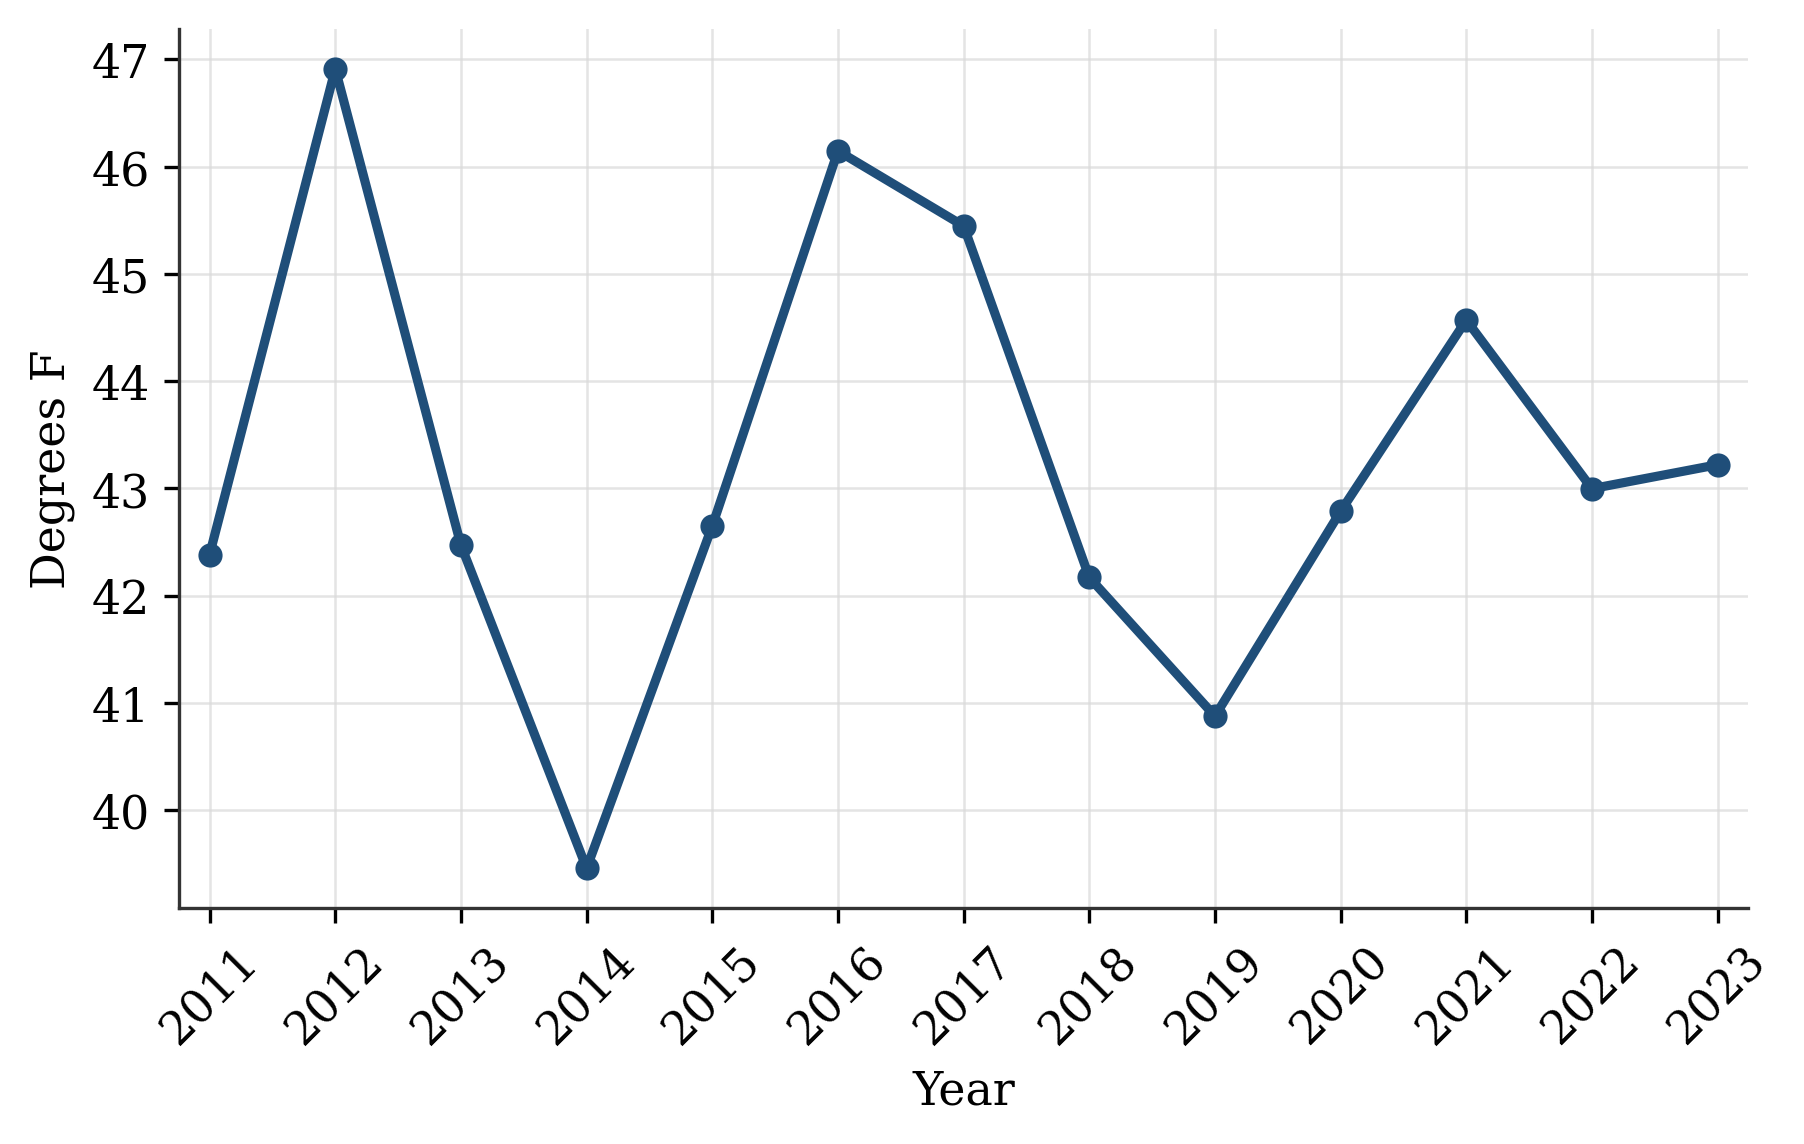
\includegraphics[width=\textwidth]{../output/figures/avg_temp_by_year.png}
  \caption{Average temperature by year}
\end{subfigure}
\hfill
\begin{subfigure}[t]{0.48\textwidth}
  \centering
  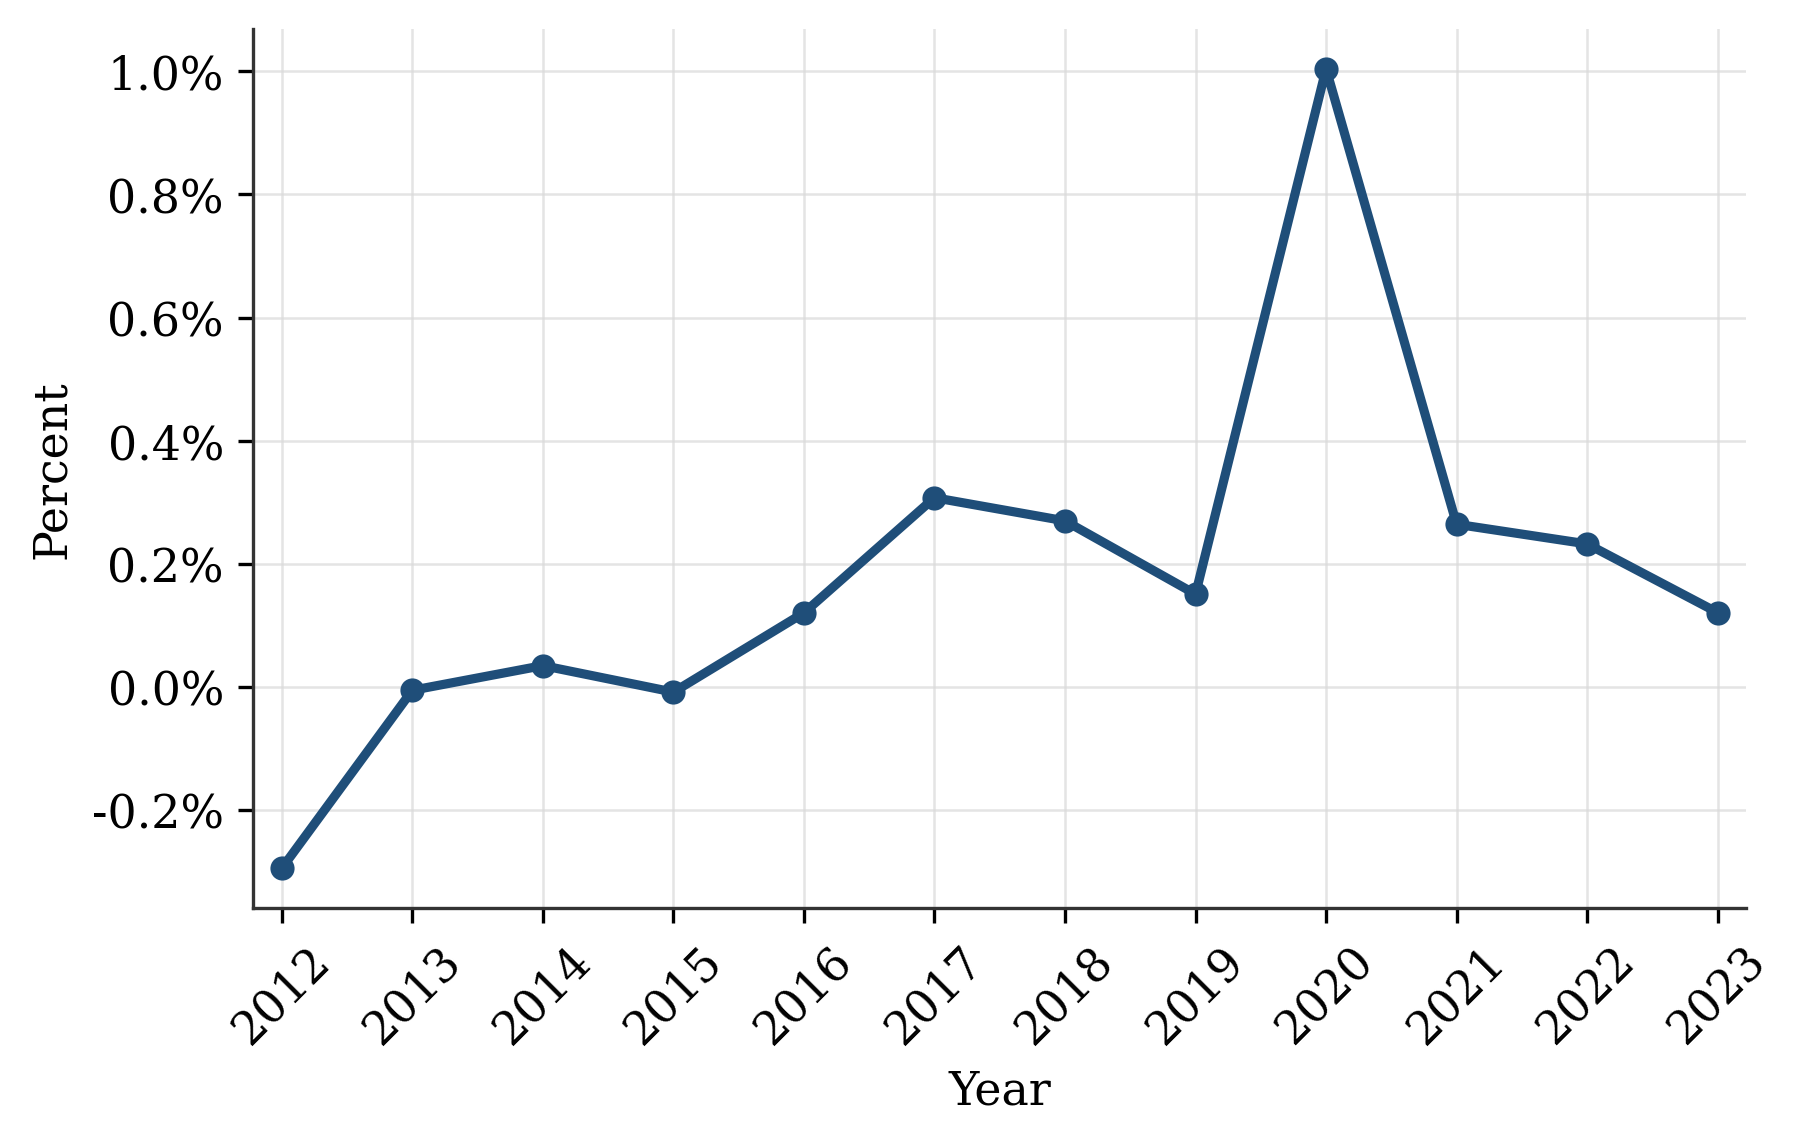
\includegraphics[width=\textwidth]{../output/figures/avg_pop_growth_by_year.png}
  \caption{Average population growth by year}
\end{subfigure}

\medskip

\begin{subfigure}[t]{0.48\textwidth}
  \centering
  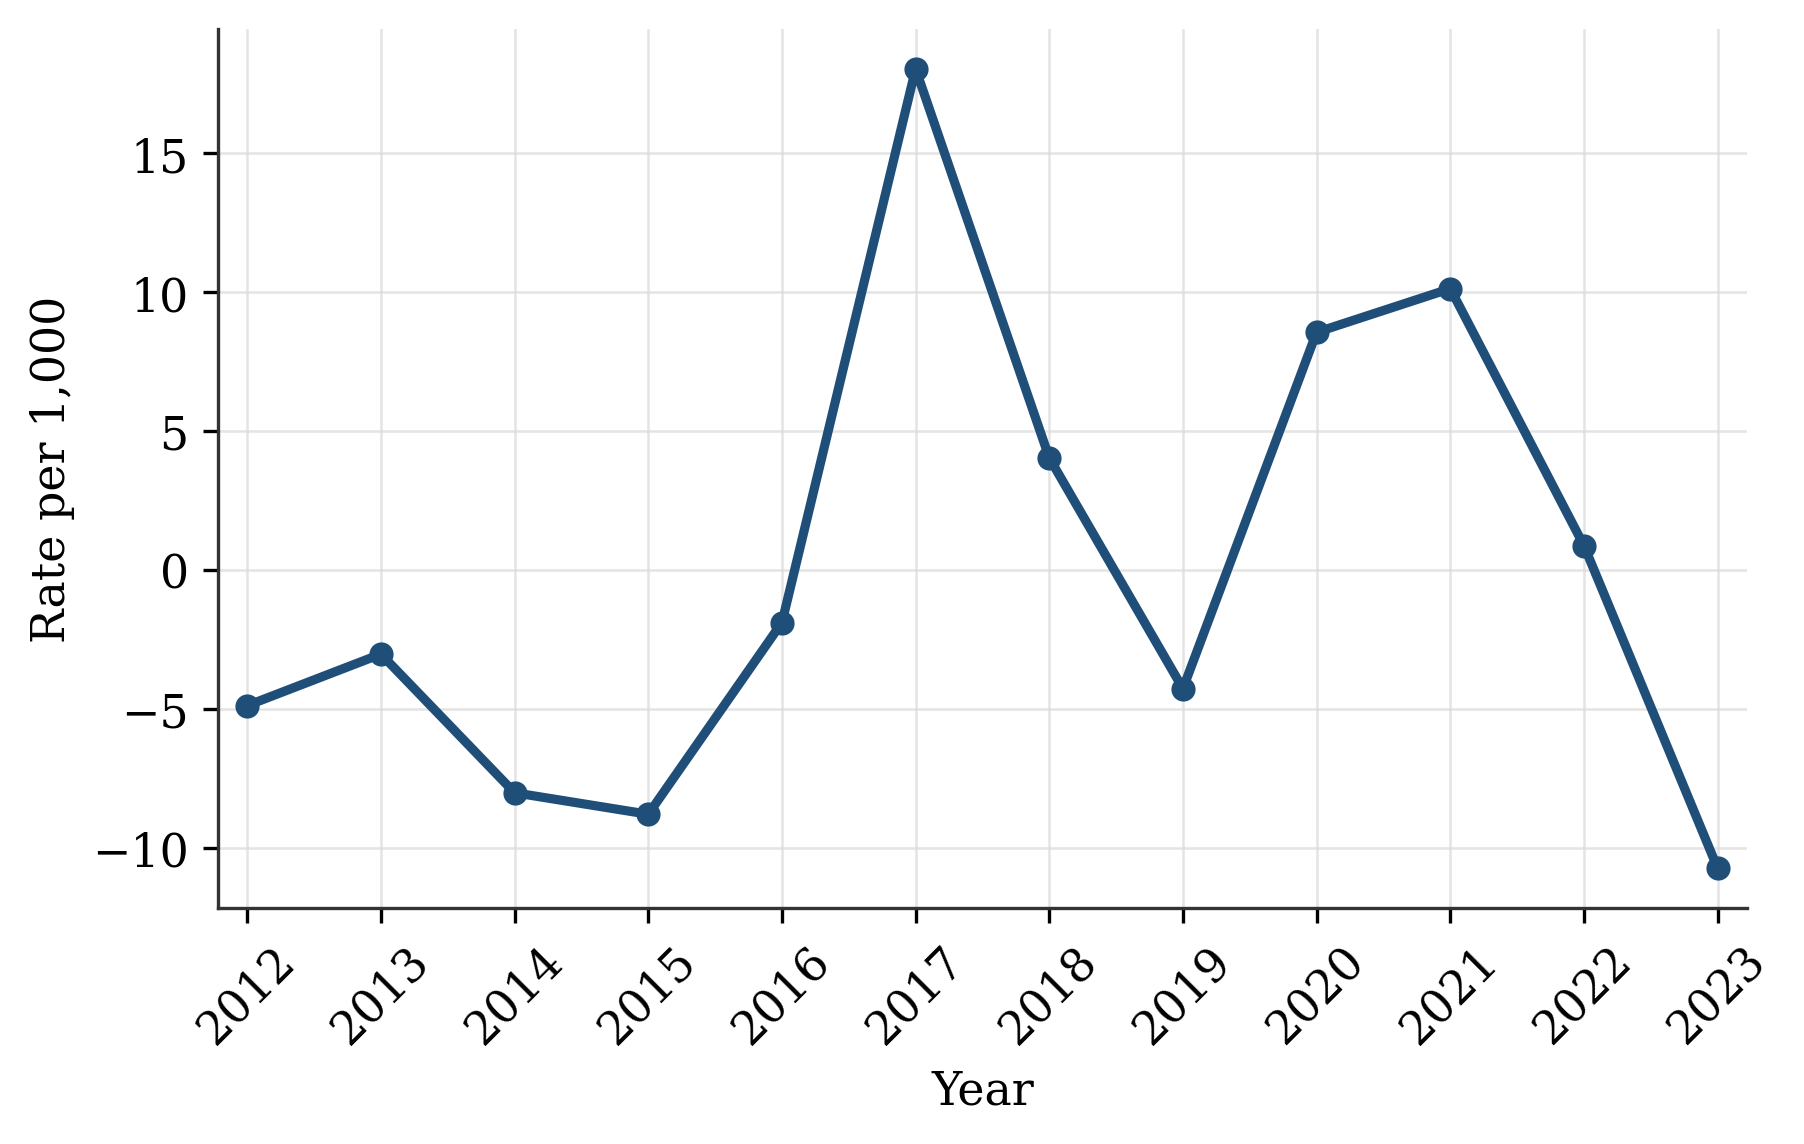
\includegraphics[width=\textwidth]{../output/figures/avg_irs_net_mig_rate_by_year.png}
  \caption{Average IRS net migration rate by year}
\end{subfigure}
\hfill
\begin{subfigure}[t]{0.48\textwidth}
  \centering
  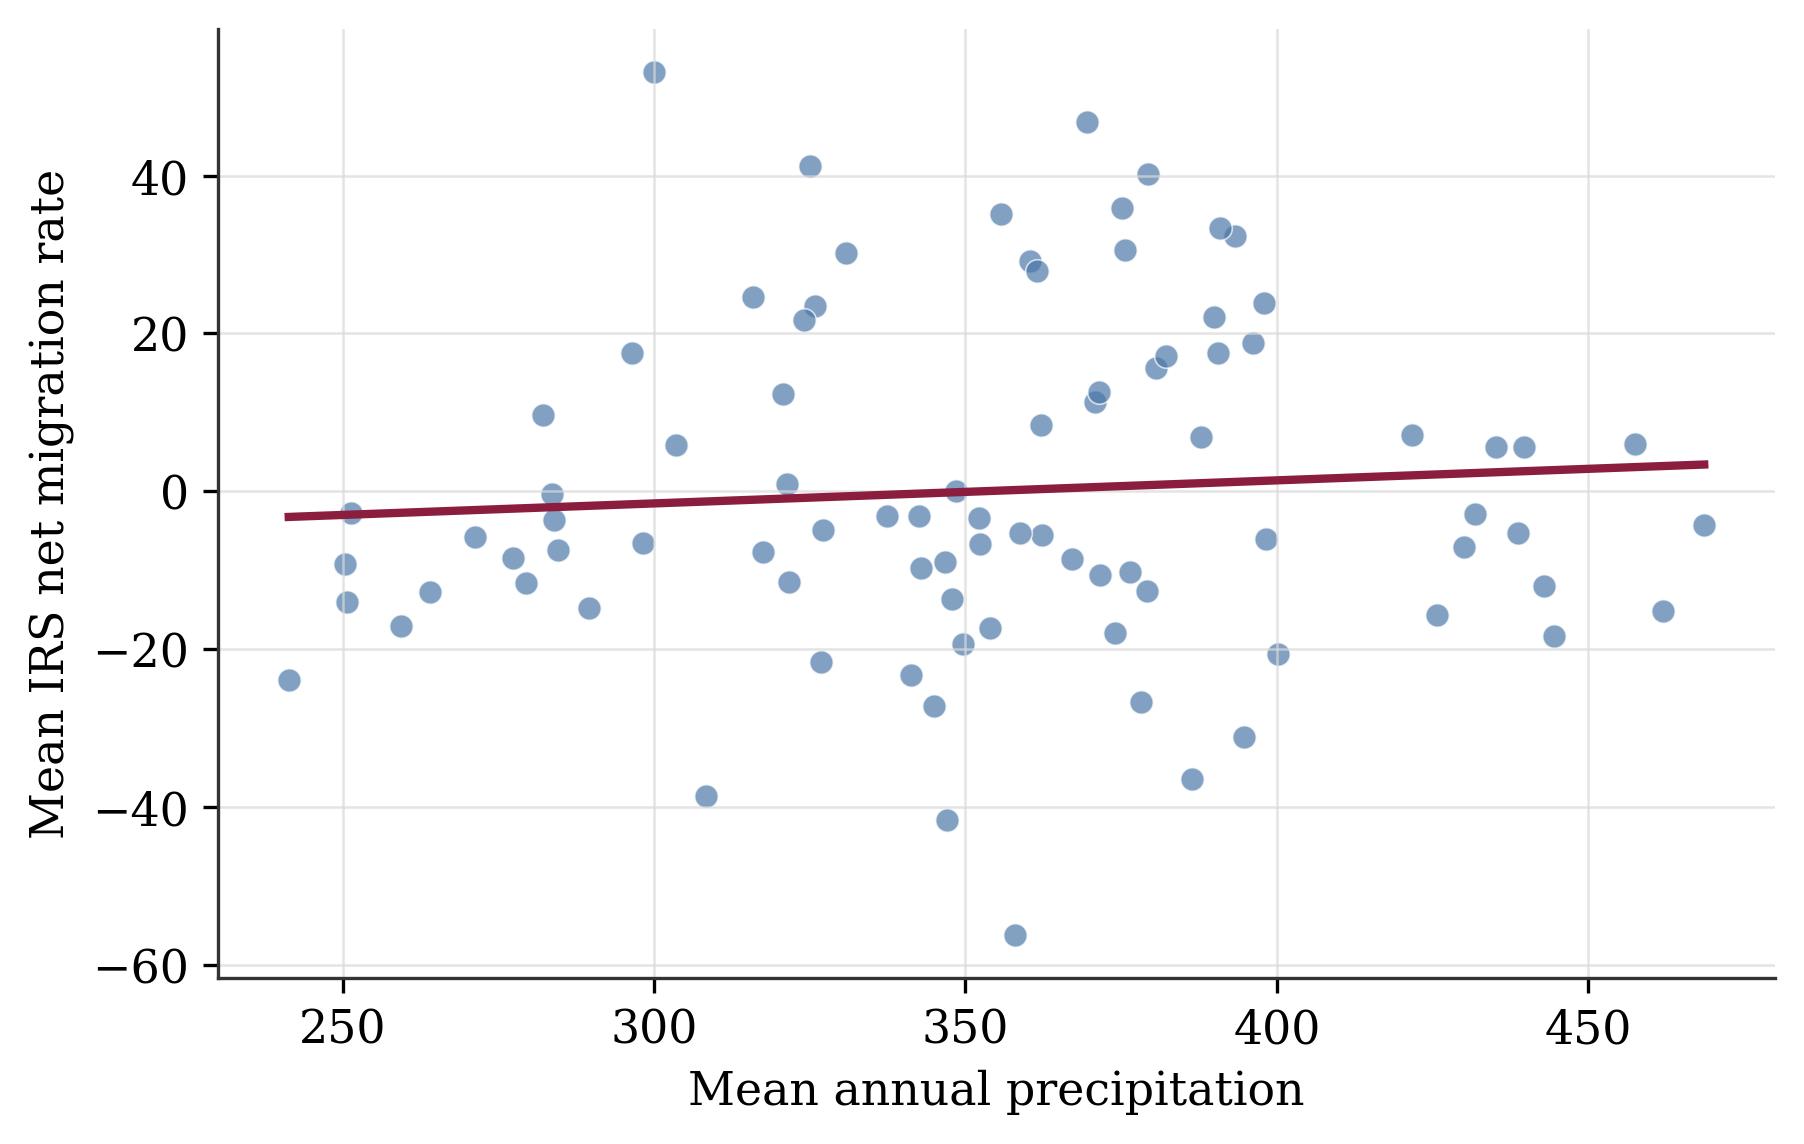
\includegraphics[width=\textwidth]{../output/figures/county_mean_irs_net_mig_vs_precip_lfit.png}
  \caption{County mean IRS net migration and precipitation}
\end{subfigure}
\caption{Statewide average temperature, population growth, and IRS net migration over time, together with the county-level relationship between mean precipitation and mean IRS net migration.}
\label{fig:descriptive}
\end{figure}

\begin{table}[htbp]
\centering
\caption{Summary of Main Empirical Patterns}
\label{tab:summary_patterns}
{\small
\setlength{\tabcolsep}{4pt}
\begin{tabular}{@{}L{1.55in}L{1.35in}L{2.65in}@{}}
\toprule
Outcome family & Dominant weather margin & Main pattern \\
\midrule
Permit units & Precipitation & Building permit units fall in wetter county-years across contemporaneous, lagged, and moving-average specifications. \\
Construction GDP & Precipitation & Total GDP is muted, but construction GDP is lower in wetter county-years across contemporaneous and persistent specifications. \\
Crop yields & Precipitation & Corn and soybean yields fall in wetter county-years, while planted acreage is much less responsive. \\
Construction establishments & Precipitation & Wetter county-years are associated with fewer construction establishments. \\
QWI labor flows & Precipitation & Wetter county-years are associated with lower total-private hiring, lower total-private employment, and higher construction separation rates. \\
Employment & Precipitation & Employment is lower in wetter county-years, especially in lagged and multi-year specifications. \\
Population growth & Precipitation & Wetter county-years are associated with slower population growth. \\
IRS net migration & Precipitation & Wetter county-years are associated with weaker net migration, mainly through lower inflows. \\
Unemployment & Mixed & Unemployment does not cleanly mirror employment, suggesting adjustment through migration and labor-force composition. \\
Per capita income & Temperature & Hotter county-years are associated with lower per capita income, especially in lagged and moving-average specifications. \\
Total personal income & Temperature and precipitation & Total income is lower with higher temperature and higher precipitation. \\
\bottomrule
\end{tabular}
}
\end{table}

Figure~\ref{fig:extension_coeffs} summarizes two of the most useful extensions to the baseline evidence. The left panel collects precipitation coefficients across several log outcomes and shows that the negative effects are concentrated in employment, permitting, construction establishments, construction GDP, and crop yields. The right panel shows that the NASS yield results are not purely contemporaneous: the precipitation coefficients remain negative in one-year-lag and three-year moving-average specifications for both corn and soybeans.

\begin{figure}[htbp]
\centering
\begin{subfigure}[t]{0.48\textwidth}
  \centering
  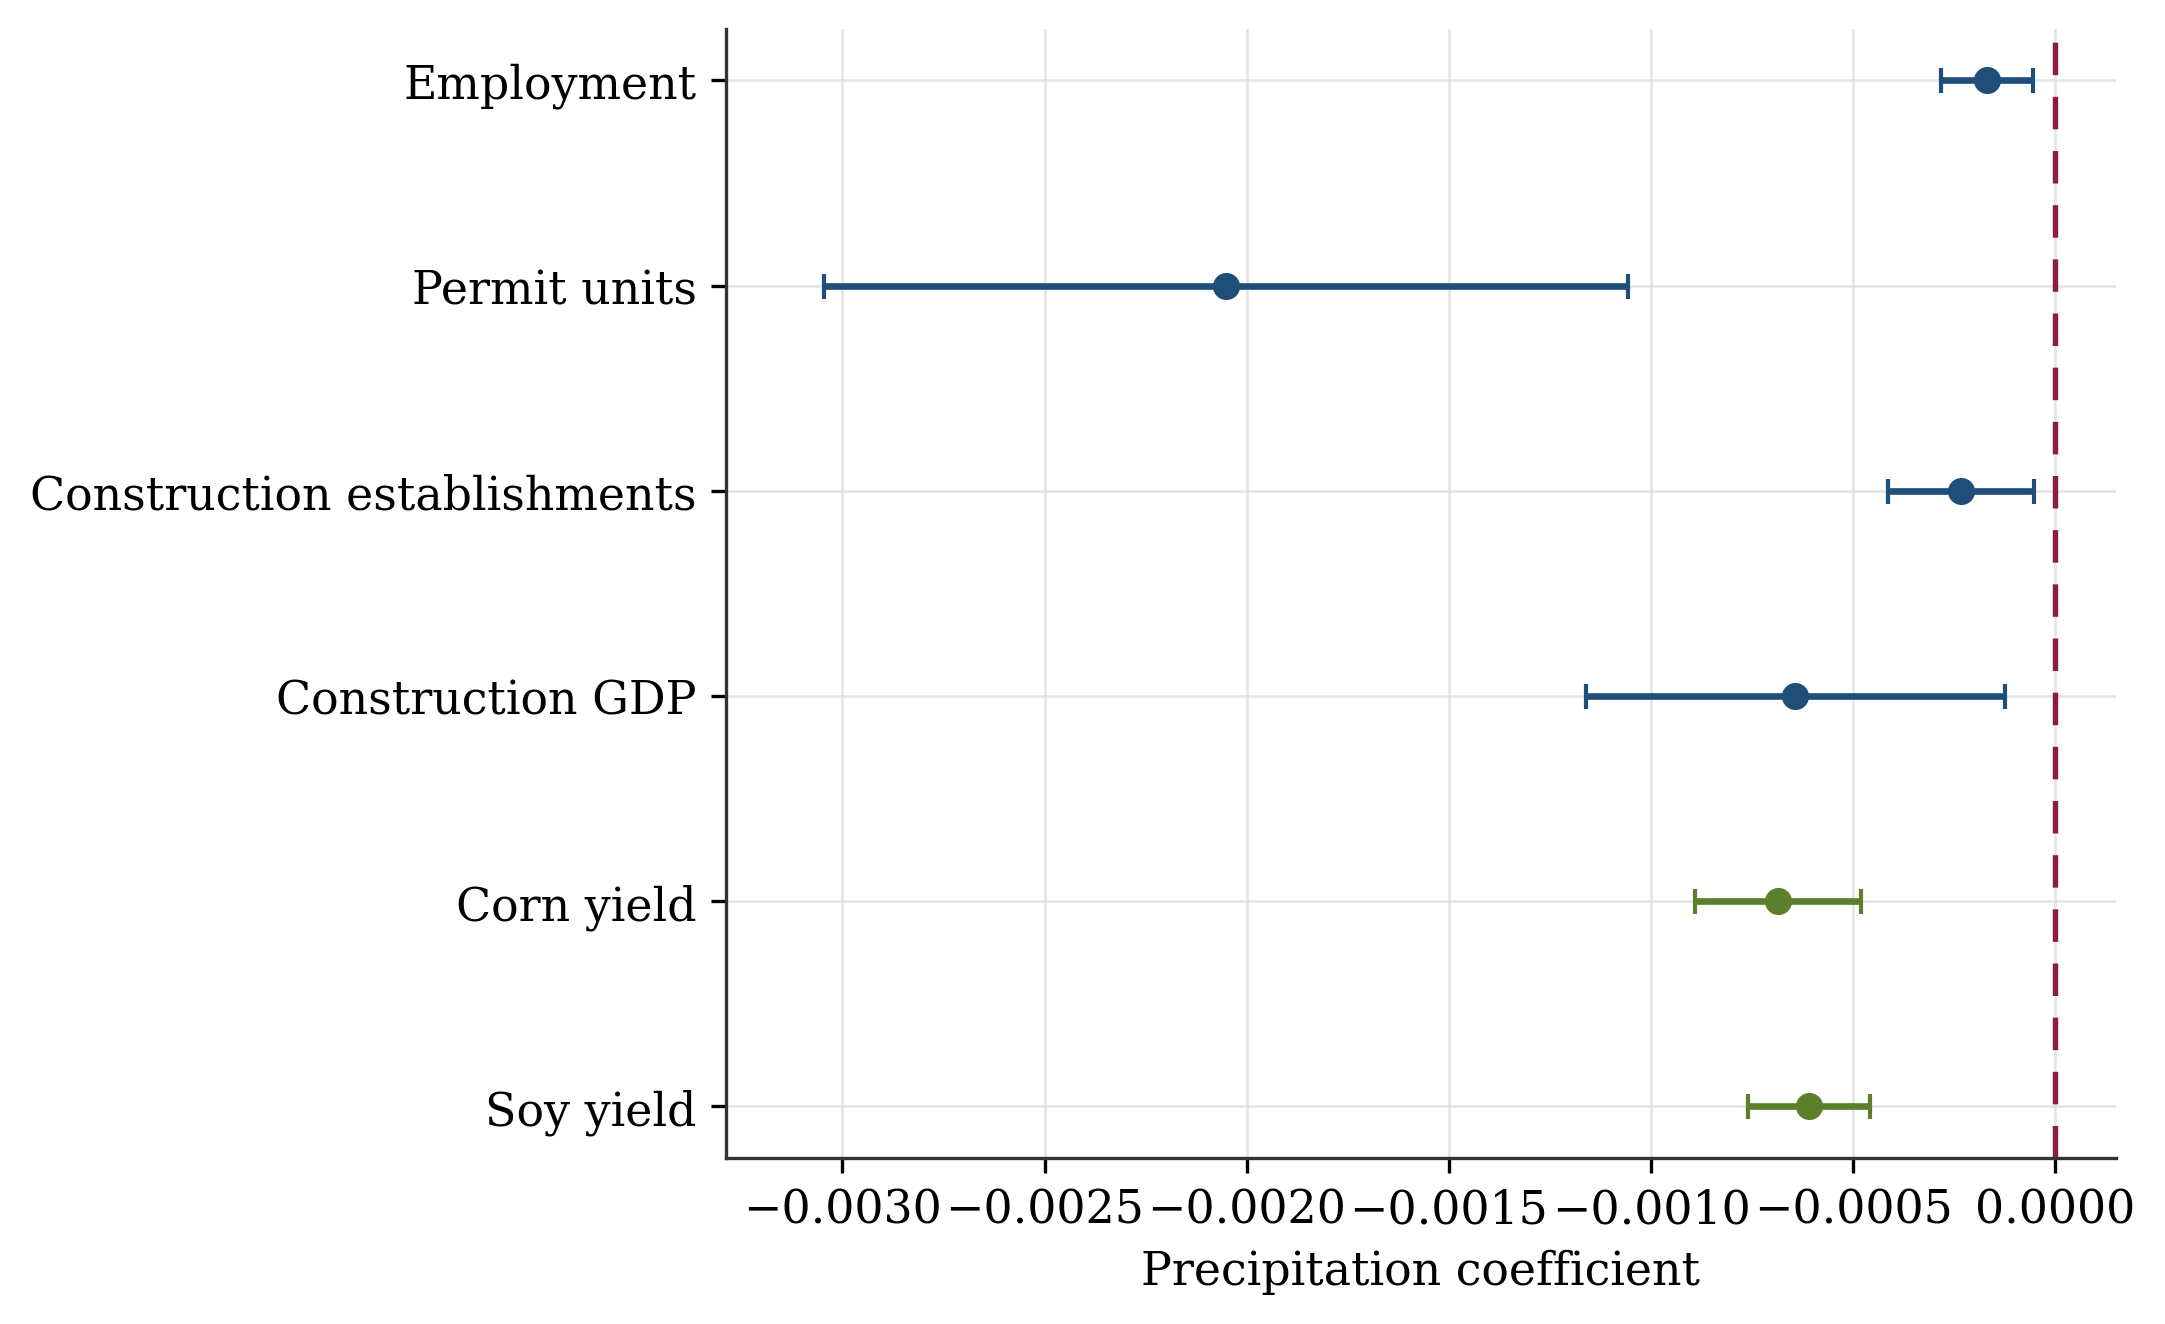
\includegraphics[width=\textwidth]{../output/figures/working_paper_precip_log_outcomes.png}
  \caption{Precipitation effects across key log outcomes}
\end{subfigure}
\hfill
\begin{subfigure}[t]{0.48\textwidth}
  \centering
  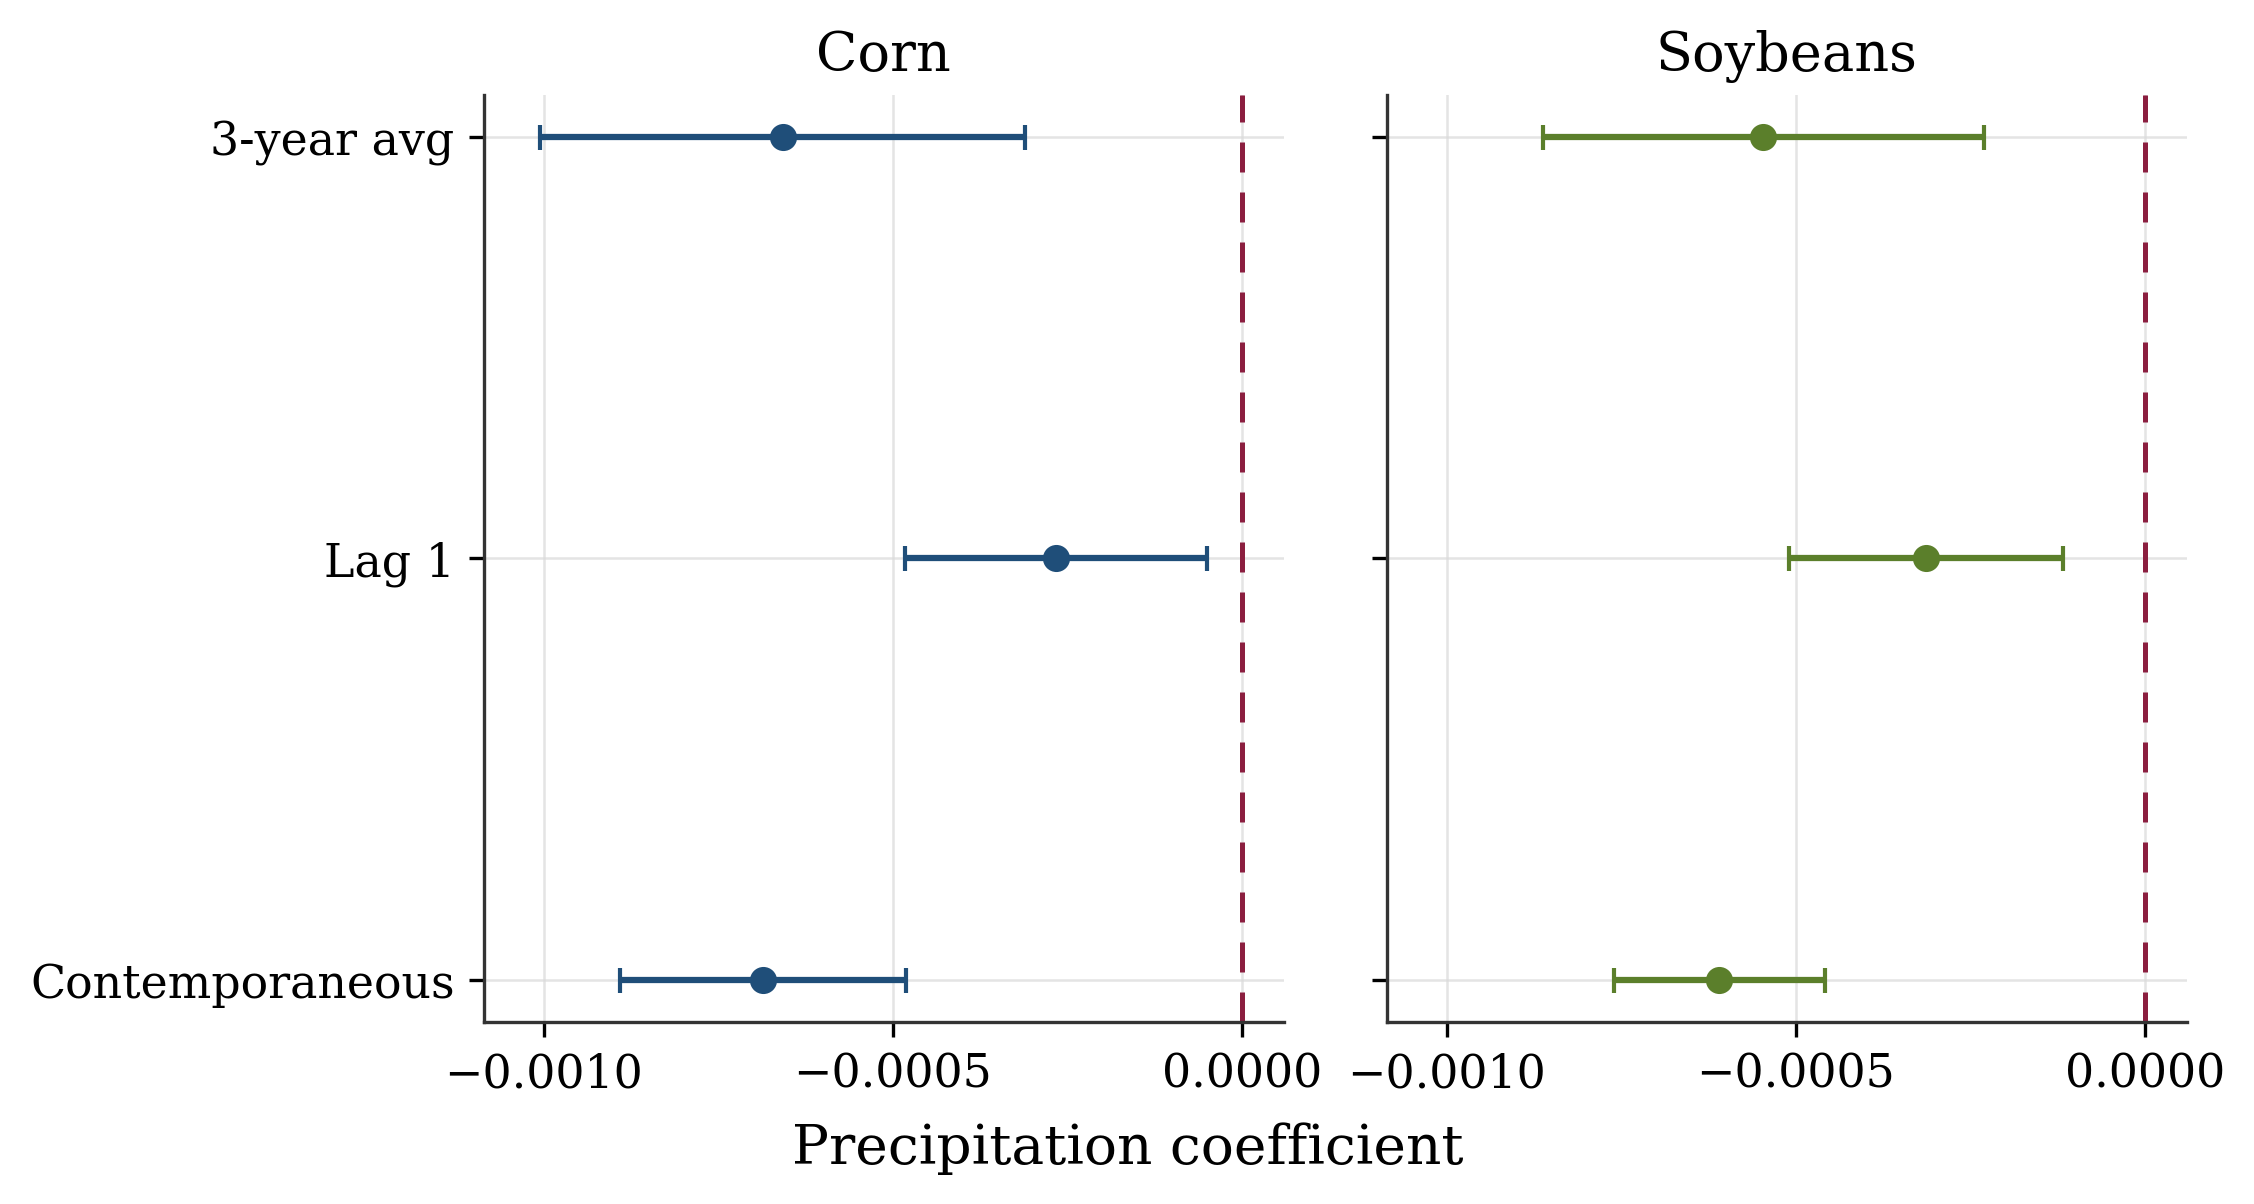
\includegraphics[width=\textwidth]{../output/figures/working_paper_nass_yield_persistence.png}
  \caption{NASS yield persistence}
\end{subfigure}
\caption{Precipitation coefficients for key log outcomes and NASS yield-persistence estimates. Points denote coefficients and whiskers denote 95 percent confidence intervals.}
\label{fig:extension_coeffs}
\end{figure}

\section{Empirical Findings}

Table~\ref{tab:baseline_results} reports the baseline county fixed-effects estimates for the paper's five headline outcomes. Precipitation enters negatively in every equation, with statistically precise baseline effects for population growth, net migration, log employment, log permit units, and log construction establishments. The table is useful as a baseline summary, but the broader results that follow place the greatest weight on permitting and on the sectoral extensions in construction GDP and crop yields, with employment interpreted more cautiously once county-specific trends are introduced.

\begin{table}[htbp]
\centering
\caption{Baseline Fixed-Effects Estimates Across Headline Outcomes}
\label{tab:baseline_results}
{\footnotesize
\setlength{\tabcolsep}{5pt}
\resizebox{\textwidth}{!}{%
\begin{tabular}{@{}L{1.3in}ccccc@{}}
\toprule
& Population growth & IRS net migration & Log QCEW employment & Log permit units & Log construction estabs \\
\midrule
Temperature & 0.0572 & 1.8409 & 0.0010 & -0.0145 & 0.0045 \\
& (0.0704) & (2.2267) & (0.0052) & (0.0491) & (0.0081) \\
Precipitation & -0.0019** & -0.0565** & -0.0002*** & -0.0021*** & -0.0002** \\
& (0.0008) & (0.0268) & (0.0001) & (0.0005) & (0.0001) \\
County fixed effects & Yes & Yes & Yes & Yes & Yes \\
Year fixed effects & Yes & Yes & Yes & Yes & Yes \\
$N$ & 1,044 & 1,044 & 1,131 & 1,131 & 1,131 \\
Within $R^2$ & 0.1323 & 0.1206 & 0.1570 & 0.1701 & 0.0448 \\
\bottomrule
\end{tabular}}

\medskip
\parbox{0.96\textwidth}{\footnotesize Notes: Standard errors clustered at the county level are in parentheses. All regressions include county and year fixed effects. * $p<0.10$, ** $p<0.05$, *** $p<0.01$.}
}
\end{table}

\subsection{Core Results: Housing and Construction}

The housing and construction evidence provides the paper's clearest headline results. In the Census Building Permits Survey, wetter county-years are associated with fewer permit units in contemporaneous, lagged, and three-year moving-average specifications. Permit values are much less informative. This difference matters because it suggests that precipitation is more clearly connected to the quantity of new construction than to reported dollar values, which are noisier and more sensitive to composition.

The implied magnitudes are large. At the sample interquartile range of annual precipitation, the baseline permit specification implies roughly 20 percent fewer permit units. That is large enough to matter for local housing supply, contractor activity, and the pace of county-level expansion.

County Business Patterns provide a complementary firm-side view of the same mechanism. Wetter county-years are associated with fewer construction establishments in the baseline, weighted, lagged, and multi-year precipitation specifications, but that equation weakens once county-specific trends are added. Construction employment, by contrast, is weaker and mostly null. That pattern indicates that the clearest construction margin in the paper is permitting, with establishment counts providing supporting but less decisive evidence.

Taken together, the permit and construction-firm results indicate that repeated wet years are associated with a thinner local construction base. That is the central local-adjustment margin in the paper.

\subsection{Core Results: Output and Agricultural Productivity}

The county GDP and agricultural extensions add the second major pillar of the paper. In BEA local GDP data, total real GDP is mostly flat with respect to the weather measures. Construction GDP, however, is lower in wetter county-years and remains negative in one-year-lag and three-year moving-average precipitation specifications. This pattern lines up closely with the permitting results. It suggests that the local output effects of wet conditions are concentrated in sectors tied to building activity rather than spread uniformly across all county production.

The NASS crop regressions provide a second, distinct piece of mechanism-consistent evidence. Wetter county-years are associated with significantly lower corn and soybean yields in contemporaneous, lagged, and three-year moving-average specifications. The yield results are among the strongest in the paper: they are statistically precise, economically meaningful, and consistent across both major Minnesota crops. By contrast, planted acreage responses are much weaker. Corn planted acreage is mostly noisy and in some persistence specifications even positive, while soybean acreage is more responsive to temperature than to precipitation. The core implication is that wet conditions show up much more clearly as a productivity shock than as a broad withdrawal of planted land.

The baseline magnitudes are substantial. At the sample interquartile range of annual precipitation, the estimates imply about 6.7 percent lower construction GDP, 7.1 percent lower corn yields, and 6.4 percent lower soybean yields. Those are large enough to make the sectoral and agricultural channels central to the paper rather than auxiliary robustness checks.

This combination of lower construction output and lower crop productivity is the paper's most durable evidence that repeated wet years matter economically in this setting.

\subsection{Supporting Evidence: Labor-Market Adjustment}

The labor-market evidence reinforces the precipitation story, but in a more qualified way than the construction and output results. Employment levels are lower in wetter county-years, and the relationship is strongest in lagged and multi-year precipitation specifications. In the baseline fixed-effects model, moving from the 25th to the 75th percentile of annual precipitation in the sample is associated with about 1.8 percent lower county employment.

That said, the employment equation is not among the paper's most stable headline results. The negative coefficient survives in the baseline and population-weighted regressions, but it attenuates to essentially zero once county-specific linear trends are added. I therefore interpret the employment block as supporting evidence of local labor-market strain rather than as a central empirical pillar.

The QWI extensions help interpret what sits underneath that pattern. In the total-private sector, wetter county-years are associated with lower hiring and lower employment. In construction, the clearest QWI response is not a uniform collapse in employment levels but a rise in separation rates. This suggests that wet conditions disrupt local labor demand partly by slowing expansion in the broader private sector and partly by raising churn and job destruction pressure in construction.

The flood-risk heterogeneity results are clearest in the employment equations. The negative relationship between precipitation and employment becomes stronger in counties with higher inland flood risk. That pattern is visible even though the level effect itself is more fragile under county trends, which makes the interaction result more informative than the baseline employment coefficient alone.

\subsection{Supporting Evidence: Demographic Adjustment}

The demographic results move in the same direction, but they are more fragile than the core construction and productivity results. In county fixed-effects models, precipitation is negatively associated with both population growth and IRS net migration. Temperature is not a robust predictor of either outcome in the longer panel.

The migration decompositions suggest that wetter county-years are more clearly associated with lower in-migration than with higher out-migration. This matters because it points to weaker attraction rather than dramatic place abandonment. If fewer households move in, local demand, labor supply, and housing absorption can all weaken over time.

At the same time, the robustness checks sharply limit how much weight the paper should place on the demographic block. In county-trend specifications, the precipitation effect on population growth remains negative, but the IRS net migration coefficient becomes less precise. Population-weighted regressions likewise make the migration results less stable than the construction and sectoral-output results. I therefore treat the demographic evidence as supporting context rather than a central headline contribution.

\subsection{Supplementary Results: Income and Wages}

The income results add an important dimension because they show that temperature is not irrelevant; it simply operates most clearly in broader income measures rather than in the core construction or productivity equations. BEA per capita income is lower in hotter county-years, and the temperature relationship becomes stronger in lagged and moving-average specifications. Total personal income is lower in counties and years with both higher temperatures and higher precipitation.

These findings matter because they show why average wage regressions alone can be misleading. In the Minnesota data, wage levels are among the weakest outcome families. They do not consistently capture the weather-economy relationship. Broader income measures, however, indicate that household economic well-being is still affected, especially through temperature. This is useful supplementary evidence, but it is not as central to the paper as the permitting, construction-GDP, and crop-yield results.

Table~\ref{tab:selected_mechanisms} collects several of the strongest non-headline estimates in one place. The table highlights the overall pattern that drives the paper's preferred interpretation: wetter county-years are associated with weaker hiring, higher construction separations, lower construction GDP, and lower crop yields, even though the evidence is not being presented as a formal mediation exercise.

\begin{table}[htbp]
\centering
\caption{Selected Mechanism-Consistent Estimates}
\label{tab:selected_mechanisms}
{\footnotesize
\resizebox{\textwidth}{!}{%
\begin{tabular}{@{}lccccc@{}}
\toprule
& Total-private hires & Construction sep. rate & Construction GDP & Corn yield & Soybean yield \\
\midrule
Temperature & -0.0100 & 0.6699 & -0.0404* & 0.0031 & -0.0244* \\
& (0.0116) & (1.3420) & (0.0230) & (0.0119) & (0.0135) \\
Precipitation & -0.0002* & 0.0461*** & -0.0006** & -0.0007*** & -0.0006*** \\
& (0.0001) & (0.0128) & (0.0003) & (0.0001) & (0.0001) \\
County fixed effects & Yes & Yes & Yes & Yes & Yes \\
Year fixed effects & Yes & Yes & Yes & Yes & Yes \\
$N$ & 1,131 & 1,106 & 1,095 & 913 & 910 \\
Within $R^2$ & 0.1842 & 0.2611 & 0.0453 & 0.5525 & 0.5111 \\
\bottomrule
\end{tabular}}

\medskip
\parbox{0.96\textwidth}{\footnotesize Notes: The table reports selected contemporaneous specifications drawn from the broader mechanism and sectoral blocks. Standard errors clustered at the county level are in parentheses. All regressions include county and year fixed effects. * $p<0.10$, ** $p<0.05$, *** $p<0.01$.}
}
\end{table}

\subsection{Synthesis Across Outcomes}

Across the outcome families, the most coherent interpretation is that precipitation is the dominant adverse weather margin for local real activity in Minnesota. The most persuasive evidence is concentrated in permitting, construction-sector output, and agricultural yields. Wetter county-years are also associated with weaker construction-establishment counts and weaker QWI hiring margins, while the demographic and employment blocks move in the same direction less consistently. Temperature matters, but primarily through broader income measures and some acreage responses rather than through the headline real-activity margins.

This synthesis is exactly what the layered econometric framework was designed to test. The baseline fixed-effects equations identify the broad weather-outcome relationships. The lag and moving-average equations show that the precipitation effect is persistent rather than purely contemporaneous. The interaction equations show that precipitation is more harmful for employment in counties with higher inland flood risk. The mechanism-oriented equations organize the evidence into a county-economy narrative in which weather stress shows up most clearly in building activity and productivity, with labor and demographic outcomes providing secondary evidence of broader adjustment.

\section{Interpretation, Identification, and Scope}

The estimates in this paper should be interpreted as within-county associations between annual weather conditions and local outcomes after absorbing county and year fixed effects. This is a strong design for a county-year panel, but it is not a randomized experiment. The paper therefore does not claim that every coefficient recovers a structural causal parameter in the narrowest sense. What it does claim is that the empirical pattern is coherent across multiple outcome families and consistent with a specific local adjustment narrative.

That coherence is important. A single negative precipitation coefficient in one table could be noise. But a repeated pattern in permits, construction GDP, crop yields, and several supporting labor and demographic equations is harder to dismiss. The fact that the results line up most clearly around precipitation, and that flood-risk heterogeneity appears where theory would most naturally predict it, strengthens the case that the paper is capturing meaningful local adjustment under repeated wet years rather than arbitrary statistical fluctuation.

The new robustness exercises also clarify where the paper is strongest and where it should remain cautious. One-year lead placebo models are close to null for population growth, IRS net migration, and construction establishments, but future precipitation still predicts QCEW employment and permit units. That is a genuine warning sign rather than a result to explain away, and it means the employment and permitting equations should not be presented as cleanly isolated causal effects. County-specific linear trends preserve the negative precipitation results for population growth and permit units but weaken the employment and construction-establishment equations considerably. This is a demanding specification because county-specific trends absorb slow-moving local growth paths, so the remaining coefficient is identified only from year-to-year deviations around each county's own trajectory. Population-weighted regressions leave the log employment, permit, and construction-establishment results negative, but they flip population growth positive and further weaken the demographic block. The exact pattern therefore matters: permits remain negative across the main reported robustness checks; construction establishments are negative in the baseline and weighted models but not with county trends; employment is negative in the baseline and weighted models but close to zero once county trends are added; and the migration results are the least robust overall. For that reason, the paper's strongest claims should center on permitting, construction GDP, and agricultural productivity, with the labor-market and demographic estimates treated more cautiously.

The county-year design also cannot rule out spatial spillovers across nearby places. Counties are not closed economies, and some apparent local losses may reflect the relocation of workers, firms, or building activity to nearby counties rather than a pure reduction in statewide activity. The estimates should therefore be interpreted primarily as local exposure-response relationships. They are informative about where weather stress shows up, but they do not by themselves distinguish statewide economic loss from geographic reshuffling within Minnesota.

At the same time, the paper remains disciplined about what the data can support. It does not estimate a formal migration-choice model, a construction investment Bellman equation, a mediation model that point-identifies sequential channels, or a statewide equilibrium with endogenous prices and quantities in every market. Those would be valuable future extensions. For the current project, the right level of ambition is a rigorous county fixed-effects framework with explicit theory-motivated dynamics and heterogeneity. In that sense, the paper is closer to applied local macro or reduced-form urban economics than to a fully structural quantitative geography model.

That choice is deliberate. The paper uses formal structure where it improves identification, interpretation, and coherence across outcomes, while avoiding structural assumptions that the available county-year data cannot credibly discipline.

\section{Policy and Research Implications}

The results suggest that weather-related economic pressure in Minnesota should not be understood solely as a disaster-response problem. In this paper, the clearest margins are weaker permitting, lower construction-sector output, and lower crop productivity in wetter county-years. That means resilience is also a question of local production capacity and future housing supply, not only current physical damage.

This has three practical implications. First, housing and infrastructure adaptation may have local growth effects that are larger than a narrow property-damage framework would imply. If wet conditions suppress permitting, lower construction GDP, and thin the construction business base, then adaptation can matter for future housing supply as well as current resilience. Second, agricultural adaptation matters even when acreage does not collapse. The NASS results suggest that productivity losses in corn and soybeans can accumulate through wetter conditions even without a large immediate reduction in planted land. Third, labor-market and demographic weakening may still matter, but the current evidence suggests they should be treated as secondary margins rather than as the core policy takeaway from this county-year design.

For future research, the most promising extensions would deepen rather than replace the current framework. A natural next step would be to estimate more flexible nonlinear weather effects or threshold effects around very wet years. Another extension would connect county-level housing prices to the construction margins already documented here. A more ambitious path would be to embed the reduced-form results in a formally estimated forward-looking migration or housing-investment model. But such work should build on the reduced-form patterns established in this paper, not skip over them.

\section{Conclusion}

This paper uses annual county-level weather variation to study local adjustment under existing flood exposure in Minnesota. The central empirical result is that precipitation is the most consistent adverse weather margin in the data. The strongest headline results are fewer building permits, lower construction GDP, and lower corn and soybean yields in wetter county-years. At the sample interquartile range of annual precipitation, the baseline estimates correspond to about 19.9 percent fewer permit units, 6.7 percent lower construction GDP, and 6 to 7 percent lower corn and soybean yields.

The strongest and most stable evidence lies in permit units, construction GDP, and crop yields. QWI labor-flow estimates add complementary evidence through lower total-private hiring and higher construction separation rates, while total county GDP and planted acreage remain much less responsive. Employment is negative in the baseline and weighted specifications but not once county-specific trends are added, and the demographic estimates are weaker still. The county-level design also cannot by itself rule out spatial reshuffling across nearby places. Even with those limitations, the paper shows that repeated wet years in a flood-exposed inland state are most clearly associated with weaker construction activity, lower construction-sector output, and lower agricultural productivity. That narrower claim provides a useful foundation for future work on local adjustment under weather stress, housing supply, and regional adaptation.

\begin{thebibliography}{99}

\bibitem[BEA(2025a)]{bea_cainc}
Bureau of Economic Analysis. 2025a. \emph{Local Area Personal Income and Employment, CAINC1}.

\bibitem[BEA(2025b)]{bea_gdp}
Bureau of Economic Analysis. 2025b. \emph{Local Area Gross Domestic Product, CAGDP}.

\bibitem[Blanchard and Katz(1992)]{blanchard1992}
Blanchard, Olivier Jean, and Lawrence F. Katz. 1992. ``Regional Evolutions.'' \emph{Brookings Papers on Economic Activity} 23(1): 1--75.

\bibitem[BLS(2025)]{bls_laus}
Bureau of Labor Statistics. 2025. \emph{Local Area Unemployment Statistics}.

\bibitem[Burke and Emerick(2016)]{burke2016}
Burke, Marshall, and Kyle Emerick. 2016. ``Adaptation to Climate Change: Evidence from US Agriculture.'' \emph{American Economic Journal: Economic Policy} 8(3): 106--140.

\bibitem[Cattaneo and Peri(2016)]{cattaneo2016}
Cattaneo, Cristina, and Giovanni Peri. 2016. ``The Migration Response to Increasing Temperatures.'' \emph{Journal of Development Economics} 122: 127--146.

\bibitem[Dell, Jones, and Olken(2014)]{dell2014}
Dell, Melissa, Benjamin F. Jones, and Benjamin A. Olken. 2014. ``What Do We Learn from the Weather? The New Climate-Economy Literature.'' \emph{Journal of Economic Literature} 52(3): 740--798.

\bibitem[FEMA(2025)]{fema_nri}
Federal Emergency Management Agency. 2025. \emph{National Risk Index}.

\bibitem[FHFA(2025)]{fhfa_hpi}
Federal Housing Finance Agency. 2025. \emph{House Price Index at the County Level}.

\bibitem[Glaeser, Gyourko, and Saks(2005)]{glaeser2005}
Glaeser, Edward L., Joseph Gyourko, and Raven E. Saks. 2005. ``Why Have Housing Prices Gone Up?'' \emph{American Economic Review} 95(2): 329--333.

\bibitem[Hsiang(2016)]{hsiang2016}
Hsiang, Solomon. 2016. ``Climate Econometrics.'' \emph{Annual Review of Resource Economics} 8: 43--75.

\bibitem[Hsiang et al.(2017)]{hsiang2017}
Hsiang, Solomon, Robert E. Kopp, Amir S. Jina, James Rising, Michael Delgado, Shashank Mohan, D. J. Rasmussen, Robert Muir-Wood, Paul Wilson, Michael Oppenheimer, Kate Larsen, and Trevor Houser. 2017. ``Estimating Economic Damage from Climate Change in the United States.'' \emph{Science} 356(6345): 1362--1369.

\bibitem[Holmes and Sieg(2014)]{holmes2014}
Holmes, Thomas J., and Holger Sieg. 2014. ``Structural Estimation in Urban Economics.'' Prepared for the \emph{Handbook of Regional and Urban Economics}.

\bibitem[IRS(2025)]{irs_migration}
Internal Revenue Service. 2025. \emph{Statistics of Income County-to-County Migration Data}.

\bibitem[NASS(2025)]{nass_quickstats}
U.S. Department of Agriculture, National Agricultural Statistics Service. 2025. \emph{Quick Stats County Crop Data}.

\bibitem[NCEI(2025)]{ncei_climate}
U.S. National Centers for Environmental Information. 2025. \emph{NOAA Climate at a Glance}.

\bibitem[Saiz(2010)]{saiz2010}
Saiz, Albert. 2010. ``The Geographic Determinants of Housing Supply.'' \emph{Quarterly Journal of Economics} 125(3): 1253--1296.

\bibitem[Schlenker and Roberts(2009)]{schlenker2009}
Schlenker, Wolfram, and Michael J. Roberts. 2009. ``Nonlinear Temperature Effects Indicate Severe Damages to U.S. Crop Yields under Climate Change.'' \emph{Proceedings of the National Academy of Sciences} 106(37): 15594--15598.

\bibitem[U.S. Census Bureau(2025a)]{census_qwi}
U.S. Census Bureau. 2025a. \emph{Quarterly Workforce Indicators}.

\bibitem[U.S. Census Bureau(2025b)]{census_bps}
U.S. Census Bureau. 2025b. \emph{Building Permits Survey}.

\bibitem[U.S. Census Bureau(2025c)]{census_cbp}
U.S. Census Bureau. 2025c. \emph{County Business Patterns}.

\bibitem[U.S. Census Bureau(2025d)]{census_pop}
U.S. Census Bureau. 2025d. \emph{County Population and Housing Unit Estimates}.

\end{thebibliography}

\appendix

\section{Main Outcome Families Used in the Paper}

The paper's empirical sections are organized around the following county-year outcomes:
\begin{itemize}[leftmargin=1.2em]
\item Population growth and total population from Census county estimates.
\item IRS net migration, inflows, and outflows from county migration files.
\item Unemployment rates from BLS local area unemployment statistics.
\item Employment and wages from QCEW.
\item Hiring, separations, job gains, and job losses from QWI annual county-sector files.
\item Personal income and per capita income from BEA CAINC1.
\item Total real GDP, nominal GDP, and construction-sector GDP from BEA county GDP files.
\item Permit units and permit values from the Census Building Permits Survey.
\item Construction establishments, construction employment, and construction payroll from County Business Patterns.
\item County crop yields and planted acreage from USDA NASS, especially for corn and soybeans.
\end{itemize}

\section{Notes on Empirical Interpretation}

Three points are especially important for interpreting the equations in the main text.
\begin{enumerate}[leftmargin=1.4em]
\item Time-invariant FEMA risk measures are absorbed by county fixed effects, so only their interactions with time-varying weather variables are identified in the fixed-effects regressions.
\item The mechanism system is a conceptual map rather than a claim of point-identified causal mediation. The paper uses reduced-form evidence across multiple outcome families to evaluate whether the pattern is consistent with weather stress operating through migration, construction, labor-market flows, and agricultural productivity.
\item The dynamic law of motion is interpretive rather than fully structural. It motivates the empirical importance of lagged and moving-average weather exposure, but it is not presented as a calibrated statewide equilibrium model.
\end{enumerate}

\section{Summary of Supplemental Outcome Results}

The broader outcome blocks use the same county fixed-effects, year fixed-effects, clustered standard-error framework described in Section 3. Their substantive results can be summarized as follows:
\begin{itemize}[leftmargin=1.2em]
\item Building permits: precipitation is negative and statistically significant for permit units in contemporaneous, one-year lag, and three-year moving-average specifications. Permit values are weaker and generally not robust.
\item Construction establishments: County Business Patterns show fewer construction establishments in wetter county-years across baseline, weighted, lagged, and multi-year precipitation specifications, but the county-trend version is much weaker.
\item Construction employment: the CBP construction employment equations are weaker and mostly null, suggesting that the firm-count margin is more informative than payroll employment in this setting.
\item QWI labor flows: total-private hiring and employment are lower in wetter county-years, while construction-sector separation rates rise more clearly than construction-sector employment falls.
\item BEA GDP: total county GDP is comparatively muted, but construction GDP is lower in wetter county-years in contemporaneous, lagged, and moving-average precipitation specifications.
\item NASS agriculture: corn and soybean yields are lower in wetter county-years across contemporaneous, lagged, and moving-average specifications, while acreage responses are much weaker and less uniform.
\item BEA income: per capita income is lower in hotter county-years, especially in lagged and moving-average specifications. Total personal income is lower with both higher temperature and higher precipitation.
\item Robustness: county-trend and population-weighted checks preserve the strongest precipitation results for permits, construction GDP, and crop yields, while employment weakens materially with county trends and demographic estimates become less stable.
\end{itemize}

\section{Selected Regression Tables}

\begin{table}[htbp]
\centering
\caption{QWI Mechanism Estimates}
\label{tab:qwi_mechanisms}
\resizebox{\textwidth}{!}{%
\begin{tabular}{@{}lcccccc@{}}
\toprule
& Total-private hires & Total-private sep. rate & Total-private employment & Construction hires & Construction sep. rate & Construction employment \\
\midrule
Temperature & -0.0100 & 0.9234* & -0.0122 & -0.0145 & 0.6699 & -0.0013 \\
& (0.0116) & (0.5481) & (0.0077) & (0.0242) & (1.3420) & (0.0174) \\
Precipitation & -0.0002* & 0.0070 & -0.0002*** & 0.0002 & 0.0461*** & -0.0002 \\
& (0.0001) & (0.0048) & (0.0001) & (0.0002) & (0.0128) & (0.0002) \\
County fixed effects & Yes & Yes & Yes & Yes & Yes & Yes \\
Year fixed effects & Yes & Yes & Yes & Yes & Yes & Yes \\
$N$ & 1,131 & 1,131 & 1,131 & 1,094 & 1,106 & 1,131 \\
Within $R^2$ & 0.1842 & 0.1975 & 0.0831 & 0.0457 & 0.2611 & 0.2519 \\
\bottomrule
\end{tabular}}

\medskip
\parbox{0.96\textwidth}{\footnotesize Notes: Standard errors clustered at the county level are in parentheses. All regressions include county and year fixed effects. * $p<0.10$, ** $p<0.05$, *** $p<0.01$.}
\end{table}

\begin{table}[htbp]
\centering
\caption{NASS Yield Persistence Estimates}
\label{tab:nass_yield_persistence}
\resizebox{\textwidth}{!}{%
\begin{tabular}{@{}lcc@{}}
\toprule
Specification & Corn yield & Soybean yield \\
\midrule
Contemporaneous precipitation & -0.0007*** & -0.0006*** \\
& (0.0001) & (0.0001) \\
One-year lag precipitation & -0.0003** & -0.0003*** \\
& (0.0001) & (0.0001) \\
Three-year avg. precipitation & -0.0007*** & -0.0005*** \\
& (0.0002) & (0.0002) \\
Contemporaneous $N$ / Within $R^2$ & 913 / 0.5525 & 910 / 0.5111 \\
Lagged $N$ / Within $R^2$ & 841 / 0.4971 & 836 / 0.4490 \\
MA(3) $N$ / Within $R^2$ & 768 / 0.5088 & 763 / 0.4528 \\
\bottomrule
\end{tabular}}

\medskip
\parbox{0.96\textwidth}{\footnotesize Notes: Each row reports the precipitation coefficient from a separate fixed-effects regression for the indicated persistence specification. The contemporaneous, lagged, and moving-average equations each include the corresponding temperature measure, along with county and year fixed effects. Standard errors clustered at the county level are in parentheses. * $p<0.10$, ** $p<0.05$, *** $p<0.01$.}
\end{table}

\begin{table}[htbp]
\centering
\caption{Robustness of Precipitation Coefficients Across Headline Outcomes}
\label{tab:robustness_precip}
{\footnotesize
\begin{tabular}{@{}L{1.9in}ccc@{}}
\toprule
Outcome & Baseline FE & County trends & Population-weighted \\
\midrule
Population growth & \shortstack{-0.0019** \\ (0.0008)} & \shortstack{-0.0020** \\ (0.0009)} & \shortstack{0.0034* \\ (0.0018)} \\
IRS net migration & \shortstack{-0.0565** \\ (0.0268)} & \shortstack{-0.0348 \\ (0.0276)} & \shortstack{0.0192 \\ (0.0399)} \\
Log QCEW employment & \shortstack{-0.0002*** \\ (0.0001)} & \shortstack{-0.0000 \\ (0.0000)} & \shortstack{-0.0003*** \\ (0.0001)} \\
Log permit units & \shortstack{-0.0021*** \\ (0.0005)} & \shortstack{-0.0009* \\ (0.0005)} & \shortstack{-0.0025*** \\ (0.0005)} \\
Log construction estabs & \shortstack{-0.0002** \\ (0.0001)} & \shortstack{0.0000 \\ (0.0001)} & \shortstack{-0.0003*** \\ (0.0001)} \\
\bottomrule
\end{tabular}

\medskip
\parbox{0.94\textwidth}{\footnotesize Notes: Each cell reports the precipitation coefficient from a separate regression with county fixed effects and year fixed effects. The county-trend specification adds county-specific linear time trends. The population-weighted specification uses county population weights. Standard errors clustered at the county level are in parentheses. * $p<0.10$, ** $p<0.05$, *** $p<0.01$.}
}
\end{table}

\end{document}
